\title{Лекции по моделированию}
\chapter{Лекция 1}
\section{Расписание и формат обучения}
Приём лабораторных:\\
Среда:
15:40 - 17:15, 237л\\
17:25 - 19:00 237л\\

Суббота:
13:50 - 15:25 243л\\
15:40 - 17:15 243л\\

Модули:\\
М1: 5 неделя, минимум 12 баллов, максимум 20 баллов, одна лабораторная\\
М2: 12 неделя, минимум 12 баллов, максимум 20 баллов, две лабораторные\\
М3: 17 неделя, минимум 18 баллов, максимум 30 баллов, одна лабораторная\\

Сдано больше двух лабораторных - автомат на экзамене.

\section{Комментарии к первой лабораторной работе}
\begin{equation}
\begin{cases}
u'(x) = x^{2} + u^{2}
u(0) = 0
\end{cases}
\end{equation}

Результат:
\begin{itemize}
\item значения для $x \in [0, x_{max}]$ с заданным шагом h
\item приближения Пикара с 1 по 4 порядок
\item до второго знака после запятой - точность
\item график функции в интервале $[-x_{max}, x_{max}]$
\end{itemize}

\section{Погрешности и устойчивость}
Погрешности, возникающие при моделировании:
\begin{itemize}
\item Погрешность модели
\item Погрешность метода
\item Погрешность исходных данных
\item Погрешность округления
\end{itemize}

Устойчивость - задача называется устойчивой (корректной), если решение единственно и устойчиво по входным данныхм. Плохо обусловленная задача: $\delta y = C \delta x, C >> 0$

\section{Модели на основе ОДУ}
Все дополнительные условия заданы в одной точке - задача Коши.\\
Все дополнительные условия заданы в разных точках - краевая задача.\\

Задача Коши:\\
$u'(x) = f(x, u)$\\
$u(\xi) = \eta$\\

Решением данной задачи является сведение уравнения к производным первого порядка при помощи замены переменных:\\
$u^{n}(x) = f(x, u, u', ..., u^{n-2}, u^{n-1})$\\
$u^{(k)} = u_{k}$\\

\begin{equation}
\begin{cases}
u'_{k}=u^{(k+1)}=u_{k+1}, 0 \leqslant k \leqslant n - 2\\
u'_{n} = f(x, u_{0}, u_{1}, u_{2}, ..., u_{n-1})
\end{cases}
\end{equation}
$u_{0} \equiv u$\\
$u_{k}(\xi) = \eta_{k}, 0 \leqslant k \leqslant n - 1$\\

Методы решения:\\
\begin{itemize}
\item Аналитические
\item Приближенно аналитические
\item Численные
\end{itemize}

Для оценки точности численных методов можно использовать правило Рунге, заключающееся в том, что если мы рассчитаем функцию с шагом $h$ и $h/2$, то точность в $x_{i}$ будет выражаться как: $\frac{|y_{i, h} - y_{i, h/2}|}{2^{p} - 1}$, где p - порядок точности.

\section{Явные методы Рунге-Кутта}
$u'(x) = f(x, u)$\\
$u(\xi) = \eta$\\
$a \leqslant x \leqslant b$\\

\begin{figure}[H]
	\center{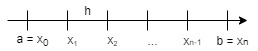
\includegraphics[scale=1.5]{a_0}}
	\caption{Значения на числовой прямой}
\end{figure}

$w_{N} = \{x_{i} : a = x_{0} < x_{1} ... < x_{N}\}$\\
$w_{n} = \{x_{i}: x_{i} = a + ih, i = \overline{0, N}\}$\\
$y_{i} \rightarrow y(x_{i})$\\

Сходимость разностного решения к точному на отрезке:\\
$\forall x_{i} \in [a, b]: |y_{i} - u_{i}| \rightarrow 0, h \rightarrow 0 (i \rightarrow \infty)$

\subsection{Метод Эйлера (p=1)}
$u_{i+1} = u_{i} + h_{i} \cdot u'_{i} + \frac{h^{2}}{2!}u''_{i}+ \frac{h^{3}}{3!}u'''_{i} + ...$\\
здесь $u'_{i} = u'(x_{i}); u''_{i} = u''(x_{i}) ...$\\
$y_{i+1} = y_{i} + h \cdot f(x_{i}, u_{i})$, если $|y_{i} - u_{i}| = o(h^{2})$, при $h \rightarrow 0$, то метод имеет p-й порядок точности.

\subsection{Численный метод Рунге-Кутта (p=2)}
$u_{i+1} = u_{i} + h u'_{i} + \frac{h^{2}}{2}u''_{i} + ...$\\
$u'_{i} = f_{i} = f(x_{i}, u_{i})$\\
$u''_{i} = (u'_{i}) = \frac{d}{dx}f = f'_{x_{i}} + f'_{u_{i}} \cdot f_{i}$\\
$y_{i+1} = y_{i} + h f_{i} + \frac{h^{2}}{2}(f'_{x_{i}} + f'_{y_{i}} \cdot f_{i}), (p=2), (2)$\\ 
$u''{i} = \frac{f(x + \gamma h, y + \delta h) - f(x, y)}{\Delta x}$\\
$y_{i+1} = y_{i} + h f_{i} + \frac{h^{2}}{2}(\frac{f(x + \gamma h, y + \delta h) - f(x, y)}{\Delta x}) = y_{i} + h[\beta f(x_{i}, y_{i}) + \alpha f (x_{i} + \gamma h, y_{i} + \delta h)]$ (3)\\
$y_{i+1} = y_{i} + h[\beta f(x_{i} + y_{i}) + \alpha (f(x_{i}, y_{i}) + f'_{x}\gamma h + f'_{y} \delta h)] = y_{i} + h[(\alpha + \beta) f(x_{i}, y_{i}) + \alpha \gamma h f'_{x} + \alpha \delta h f'_{y}]$ (4)\\

Сравним (2) и (4):\\
\begin{equation}
\begin{cases}
\alpha + \beta = 1\\
\alpha \gamma = \frac{1}{2}\\
\alpha \delta = \frac{1}{2} f(x_{i}, y_{i})\\
\end{cases}
\end{equation}

\begin{equation}
\begin{cases}
\beta = 1 - \alpha\\
\gamma = \frac{1}{2\alpha}\\
\delta = \frac{1}{2\alpha} f(x_{i}, y_{i})\\
\end{cases}
\end{equation}

Из (3) видим, что:\\
$y_{i+1} = y_{i} + h[(1 - \alpha) f(x_{i}, y_{i}) + \alpha f(x_{i} + \frac{1}{2\alpha}h, y_{i} + \frac{h}{2\alpha}f(x_{i}, y_{i}))]$, на практике $\alpha = 1, \alpha = \frac{1}{2}$\\

\subsection{Метод Пикара (приближённый аналитический метод)}
$u'(x) = f(x, u(x))$\\
$\frac{du}{dx} = f(x, u(x))$\\
$u(x) = u(\xi) + \int\limits_{\xi}^{x} f(t, u(t)) dt$\\
$y^{(\delta + 1)}(x) = u(\xi) + \int\limits_{\xi}^{x} f(t, y^{(\delta)}(t)) dt$\\% не уверен, подтвердить в интернете

В лабораторной показать Пикара нужной точности (от 1 до 4).

\chapter{Лекция 2}
$y_{n+1} = y_{n} + h_{n}[(1 - \alpha)f(x_{n}, y_{n}) + \alpha f(x_{n} + \frac{h_{n}}{2\alpha}, y_{n} + \frac{h_{n}}{2\alpha} f (x_{n}, y_{n}))] + O(max h^{2}_{n})$
\section{Геометрическое истолкование полученных результатов}
Рассмотрим для $\alpha = 1$:\\
$y_{n+1} =  y_{n} + h_{n} f(x_{n} + \frac{h_{n}}{2}, y_{n} + \frac{h_{n}}{2} f (x_{n}, y_{n}))$\\
1) $y_{n + \frac{1}{2}} = y_{n} + \frac{h_{n}}{2} f(x_{n}, y_{n})$\\
2) $y'_{n} = f(x_{n} + \frac{h_{n}}{2}, y_{n + \frac{1}{2}})$\\
3) $y_{n + 1} = y_{n} + h_{n} y'_{n}$\\
\begin{figure}[H]
	\center{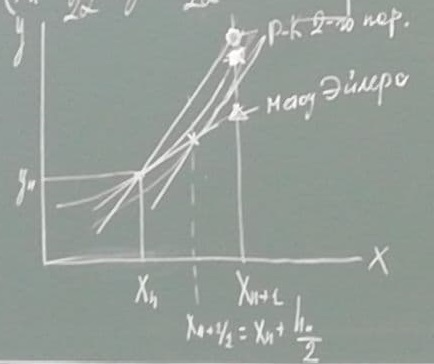
\includegraphics[scale=1.6]{a_1}}
	\caption{Геометрические результаты для a = 1}
\end{figure}

Рассмотрим для $\alpha = \frac{1}{2}$:\\
$y_{n+1} =  y_{n} + \frac{h_{n}}{2}[f(x_{n}, y_{n}) + f(x_{n} + \frac{h_{n}}{2}, y_{n} + \frac{h_{n}}{2} f (x_{n}, y_{n}))]$\\
1) $\overline{y_{n+1}} = y_{n} + h_{n} f(x_{n}, y_{n})$\\
2) $y'_{n+1} = f(x_{n} + h_{n}, \overline{y_{n+1}})$\\
3) $y'_{cp} = \frac{1}{2}(f(x_{n}, y_{n}) + y'_{n+ 1})$\\
4) $y_{n+1} = y_{n} + h_{n} \cdot y'_{cp}$
\begin{figure}[H]
	\center{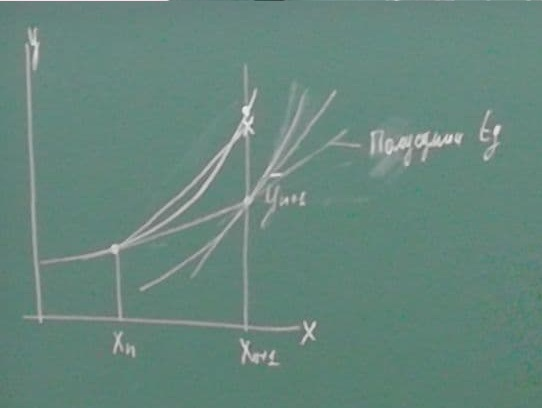
\includegraphics[scale=1.6]{a_2}}
	\caption{Геометрические результаты для a = 1/2}
\end{figure}


\section{Методы Рунге-Кутта 4-го порядка точности}
Формула обеспечивает переход из узла n в узлел n + 1:\\
$y_{n+1} = y_{n} + \frac{k_{1} + 2k_{2} + 2k_{3} + k_{4}}{6}$\\
$k_{1} = h f(x_{n}, y_{n})\\$
$k_{2} = h f (x_{n} + \frac{h}{2}, y_{n} + \frac{k_{1}}{2})$\\
$k_{2} = h f (x_{n} + \frac{h}{2}, y_{n} + \frac{k_{2}}{2})$\\
$k_{2} = h f (x_{n} + h, y_{n} + k_{3})$\\

Посмотрим, как формируется порядок точности в специальном варианте правой части:\\
$u'(x) = f(x)$\\
$y_{n+1} = y_{n} + \int\limits^{x_{n+1}}_{x_{n}}f(x) dx$\\
При $\alpha = \frac{1}{2}$\\
$y_{n+1} = y_{n} + \frac{h}{2}(f(x_{n}) + f(x_{n+1}))$\\
По методу трапеции:\\
$R_{trap} \leqslant \frac{x_{N} - x_{O}}{12} h^{2} \cdot max|f'(x)|$\\
Рунге-Кутт 4-го порядка:\\
$y_{n+1} = y_{n} + \frac{h}{6}(f(x_{n}) + 4f(x_{n} + \frac{h}{2}) + f(x_{n} + h))$ - метод Симпсона\\
$R_{simp} \leqslant \frac{x_{n} - x_{o}}{190 \cdot 16} h^{4} \cdot max|f^{IV}(x)|, x_{o} \leqslant x \leqslant x_{n}$\\

\section{Замечания о методах Рунге-Кутта}
\begin{enumerate}
\item методы явные - позволяет за строго зафиксированное количество шагов перейти из одного узла в другой
\item позволяет производить расчёты с переменным шагом
\item если нужных производынх при интегрировании нет, то применение метода Симпсона бессмысленно, т.е. метод трапеции, треугольника и тд.
\end{enumerate}

\section{Распространение метода Рунге-Кутта 4-то порядка на систему дифференциальных уравнений}
На примере метода Рунге-Кутта 4-го порядка рассмотрим распространить результат на систему дифференциальных уравнений.\\
\begin{equation}
\begin{cases}
u' = f(x, u, v)\\
v' = \phi(x, u, v)\\
u(\xi) = \eta_{1}\\
v(\xi) = \eta_{2}\\
\end{cases}
\end{equation}

$u = y, v = z$\\

$y_{n+1} = y_{n} + \frac{k_{1} + 2k_{2} + 2k_{3} + k_{4}}{6}$\\
$z_{n+1} = z_{n} + \frac{q_{1} + 2q_{2} + 2q_{3} + q_{4}}{6}$\\
$k_{1} = h f(x_{n}, y_{n}, z_{n}), q_{1} = h \phi(x_{n}, y_{n}, z_{n})$\\
$k_{2} = h f(x_{n} + \frac{h}{2}, y_{n} + \frac{k_{1}}{2}, z_{n} + \frac{q_{1}}{2}), q_{2} = h \phi(x_{n} + \frac{h}{2}, y_{n} + \frac{k_{1}}{2}, z_{n} + \frac{q_{1}}{2})$\\
$k_{3} = h f(x_{n} + \frac{h}{2}, y_{n} + \frac{k_{2}}{2}, z_{n} + \frac{q_{2}}{2}), q_{3} = h \phi(x_{n} + \frac{h}{2}, y_{n} + \frac{k_{2}}{2}, z_{n} + \frac{q_{2}}{2})$\\
$k_{4} = h f(x_{n} + \frac{h}{2}, y_{n} + \frac{k_{3}}{2}, z_{n} + \frac{q_{3}}{2}), q_{2} = h \phi(x_{n} + \frac{h}{2}, y_{n} + \frac{k_{3}}{2}, z_{n} + \frac{q_{3}}{2})$\\


Способ рассчёта выше применяется в вычислениях во второй лабораторной работе.\\

\section{Применение метода Пикара}
Возвращаясь к методу Пикара, сформулируем условие сходимости приближённого решения к точке.
\begin{itemize}
\item решение в ограниченной области
\item правая часть $f$ непрерывна
\item условия Липшеца: $a \leqslant x \leqslant b, |f(x, u_{1}) - f(x, u_{2})| \leqslant \mathcal{L}|u_{1} - u_{2}|$
\end{itemize}

\section{Неявный метод Эйлера}
$u' = f(x, u)$\\
В явном методе Эйлера - $y_{n+1} = y_{n} + h f(x_{n}, y_{n})$\\
В неявном методе Эйлера - $y_{n+1} = y_{n} + h f (x_{n + 1}, y_{n + 1})$
Последствия:\\
1) Решения может не быть, либо может быть несколько\\
2) Для решения уравнения необходимо подобрать метод\\
Применяется часто, поскольку является устойчивым.\\

Пример:\\
$u' = -\alpha u, \alpha > 0$\\
аналитическое решение: $u(x) = c e^{-\alpha x}$\\
\begin{figure}[H]
	\center{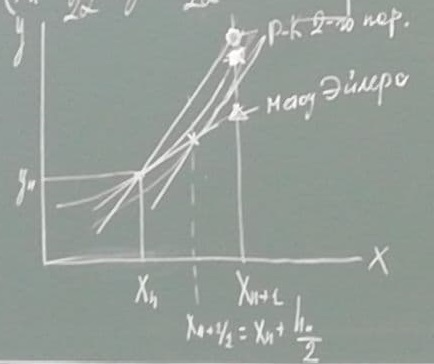
\includegraphics[scale=1.6]{a_1}}
	\caption{Сравнение явного и неявного метода Эйлера}
\end{figure}

$y_{n+1} = y_{n} - \alpha y_{n} h = y_{n} (1 - \alpha h), 1 - \alpha h > 0, h < \frac{1}{2}$\\
Применение явного метода может привести к расходящимся решениями и имеет ограничения на $\alpha$. Чем больше $\alpha$, тем больше шаг.\\

Неявный метод:\\
$y_{n+1} = y_{n} - \alpha y_{n+1}h$\\
$y_{n+1} = \frac{y_{n}}{1 + \alpha h}$ - ограничений на $h$ нет.\\

В общем виде:\\
$\sum\limits_{k=0}^{m} a_{k} y_{n - k} = h(f(x_{n}, y_{n}))$\\
$m = 1, a_{0} = 1, a_{1} = -1$\\
$y_{n} - y_{n - 1} = h f (x_{n}, y_{n})$ - метод Эйлера.\\

\section{Метод Гира}
При $m = 2$:\\
$\frac{3}{2} y_{n} - 2 y_{n-1} + \frac{1}{2}y_{n-2} = h f (x_{n}, y_{n}) + O(h^{2})$\\
При $m = 3$:\\
$\frac{11}{3}y_{n} - 3y_{n-1} + \frac{3}{2}y_{n-2} - \frac{1}{3}y_{n-3} = h f(x_{n}, y_{n}) + O(h^{3})$\\

Формул более высокого порядка точности не существует. Благоприятны с точки устойчивости решений.

\section{Замечание о многошаговых методах}
В многошаговых методах для получения решения в неизвестном узле необходимо знать значения в определённом количестве предыдущих узлов.

\chapter{Лекция 3}
\section{Методы на основе ОДУ. Краевая задача}
Дифференциальное вторение второго порядка может быть сведено к уравнению певрого порядка. В самом общем виде краевая задача формулируется следующим образом:\\
\begin{equation}
\begin{cases}
u'_{k}(x) = f_{k}(x, u_{1}, u_{2}, ..., u_{n}), k = \overline{1, n}\\
\phi_{k}(\xi_{k}, u_{1}(\xi_{k}), u_{2}(\xi_{k}), ..., u_{n}(\xi_{k})) = 0, k = \overline{1, n}
\end{cases}
\end{equation}

Методы решения:
\begin{itemize}
\item Аналитические
\item Приближённые
\item Численные
\end{itemize}

\section{Приближённый метод}
Все функции от x - заданные, надо найти u.
\begin{equation}
\begin{cases}
u'(x) + p(x)u'(x) + g(x)u(x) = f(x)\\
\alpha_{1}u'(a) + \beta_{1}u(a) = y_{1}\\
\alpha_{2}u'(a) + \beta_{2}u(a) = y_{2}\\
a \leqslant x \leqslant b\\
\end{cases}
\end{equation}

$Lu = u'(x) + p(x) u'(x) + g(x) u(x)$\\
$l_{a}u = \alpha_{1}u' + \beta_{1}u$\\
$l_{b}u = \alpha_{2}u' + \beta_{2}u$\\

\begin{equation}
\begin{cases}
Lu = f(x) (1)\\
l_{a}u = y_{1} (2.1)\\
l_{n}u = y_{2} (2.2)
\end{cases}
\end{equation}

Решение ищем в виде:\\
$y(x) = u_{0}(x) + \sum\limits_{k=1}^{n} C_{k} u_{k}(x)$\\
\begin{equation}
u_{k}(x) \rightarrow 
\begin{cases}
L_{a}u_{k} = 0\\
L_{b}u_{k} = 0
\end{cases}
\end{equation}

$R(x, C_{1}, C_{2}, ... C_{n}) = Ly - f(x) = Lu_{0}(x) + \sum\limits_{k=1}^{n} C_{k} L u_{k}(x) - f(x)$

\section{Метод коллокаций}
Выбираем множество точек $x_{i}, i = 1, ... n$\\
$R(x, C_{1}, C_{2}, ... C_{n}) = 0, i = \overline{1, n}$\\

Пример:\\
\begin{equation}
\begin{cases}
u^{n} + (1 + x^{2})u + 1 = 0\\
u(-1) = 0, u(1) = 0\\
-1 \leqslant x \leqslant 1
\end{cases}
\end{equation}

$u_{0}(x) = 0, u_{1}(x) = x^{2k - 2}(1 - x^{2}), k = 1, 2, ... n$\\
Точки коллокации - $n = 2, x_{1} = 0, x_{2} = 0.5$\\

$y(x) = C_{1} (1 - x^{2}) + C_{2} (x^{2} - x^{4})$\\
$R(x, C_{1}, C_{2}) = 1 - C_{1} (1 + x^{4}) + C_{2} (2 - 11 x^{2} - x^{6})$\\
Приравниваем полученное выше выражение к нулю в точках коллокации:\\
$x = 0, C_{1} - 2C_{2} = 1$\\
$x = 0.5, 1.0625 C_{1} + 0.7656 C_{2} = 1$\\
Решение: $C_{1} = 0.9568, C_{2} = -0.0216$\\
Окончательное решение: $y(x) = 0.1568(1 - x^{2}) - 0.0216(x_{2} - x_{4})$\\

Чем больше точек коллокация. тем лучше полученная фукнция будет совпадать с точным решением.

\section{Метод Галеркина}
$u_{0}(x), u_{1}(x), ..., u_{m}(x)$ - система ортогональных линейно-независимых функций, $a \leqslant x \leqslant b$\\
$\int\limits_{a}^{b} f(x) u_{i}(x) dx = 0, i = \overline{1, m} \Rightarrow f(x) = 0$\\
$\int\limits_{a}^{b} R(x, C_{1}, C_{2}, ..., C_{n}) u_{i} dx  = 0, i = \overline{1, m}$\\
$\int\limits_{a}^{b} u_{m} L u dx + \sum\limits_{k=1}^{n} C_{k} \int\limits_{a}^{b} u_{k} L u dx - \int\limits_{a}^{b} u_{m} f(x) dx = 0, m = 1, 2, ...n$\\

Пример:\\
\begin{equation}
\begin{cases}
u'' + x u' + u = 2x\\
u(x) = 1\\
u(1) = 0\\
0 \leqslant x \leqslant 1
\end{cases}
\end{equation}

$u_{0}(x) = 1 - x$\\
$u_{1}(x) = x^{k}(1 - x), k = 1, 2, ... n$\\
n = 3\\
$y(x) = (1 - x) + C_{1} x(1 - x) + C_{2} x^{2} (1 - x) + C_{3} x^{3} (1 - x)$\\
$R(x, C_{1}, C_{2}, C_{3}) = 1 + 3x + C_{1} (-2 + 2x - 3x^{2}) + C_{2} (2 - 6x + 3x^{2} - 4x^{4}) + C_{3} (6x - 12x^{2} + 4x^{3} - 5x^{4})$\\
Выполняя процедуру Галёркина, получим систему интегралов от трёх функций:\\
$\int\limits_{0}^{1} R(x, C_{1}, C_{2}, C_{3}) (x - x^{2}) dx = 0$\\
$\int\limits_{0}^{1} R(x, C_{1}, C_{2}, C_{3}) (x^{2} - x^{3}) dx = 0$\\
$\int\limits_{0}^{1} R(x, C_{1}, C_{2}, C_{3}) (x^{3} - x^{4}) dx = 0$\\
В результате получим систему из трёх уравнений:\\
$133 C_{1} + 63 C_{2} + 36 C_{3} = -70$\\
$140 C_{1} + 108 C_{2} + 79 C_{3} = -98$\\
$264 C_{1} + 252 C_{2} + 211 C_{3} = -210$\\
В результате получаем следующие коэффициенты: $C_{1} = -0.209, C_{2} = -0.789, C_{3} = 0.209$\\
$y(x) = (1 - x)(1 - 0.209x - 0.789 x^{2} + 0.209 x^{3})$\\

\section{Интегральный метод наименьших квадратов}
$\int\limits_{a}^{b} \Phi^{2}(x, C_{1}, C_{2}, ..., C_{n}) dx  \rightarrow min$\\
$\frac{d\Phi}{dC_{2}} = 0, \int\limits_{a}^{b} 2R(x, C_{1}, ... C_{n}) \frac{dR}{dC_{2}} dx = 0, k = 1, 2, ... n$\\
Пример:\\
Из метода коллокаций:\\
$R(x) = 1 - (1 + x^{2}) C_{2} + (2 - 11x^{2} -x^{6})C_{2}$\\
$\frac{1 d\Phi}{2 dC_{1}} = -\int\limits_{0}^{1} (1 - (1 + x^{2}) C_{1} + (2 - 11x^{2} -x^{6})C_{2}) (1 + x^{2}) dx = 0$\\
$\frac{1 d\Phi}{2 dC_{2}} = -\int\limits_{0}^{1} (1 - (1 + x^{4}) C_{1} + (2 - 11x^{2} -x^{6})C_{2}) (2 - 11x^{2} - x^{6}) dx = 0$\\
\begin{equation}
\begin{cases}
\frac{68}{45} C_{1} + \frac{3548}{1155} C_{2} = \frac{5}{4}\\
\frac{3548}{1155} C_{1} + \frac{63404}{4035} C_{2} = \frac{38}{91}
\end{cases}
\end{equation}
$C_{1} = 0.985, C_{2} = -0.078$\\
$y(x) = 0.985(1 - x^{2}) - 0.078(x^{2} - x^{4})$

\section{Дискретный метод наименьших квадратов}
$\Phi = \sum\limits_{i=1}^{N} R^{2}(x, C_{1}, C_{2}, ..., C_{n}) \rightarrow min$\\
Если взять N>>n, то метод будет работать. Если взять N = n, то метод перейдёт в метод коллокаций, надо будет показать в лабе.

\section{Метод стрельбы (численный)}
\begin{equation}
\begin{cases}
u'(x) = f(x, u, v) (3.1)\\
v'(x) = \phi(x, u, v) (3.2)\\
\Xi(u(a), v(a)) = 0 (4)\\
\psi(u(b), v(b)) = 0 (5)\\
a \leqslant x \leqslant b
\end{cases}
\end{equation}

Берем некое $u(a) = \xi$, тогда из (u):\\
$\Xi(\xi, u(a)) = 0 \rightarrow v(a) = \gamma(\xi)$\\
Сводится к задаче Коши, решаем уравнение численно\\
Например, если краевое условие - линейное, то $\alpha_{1} u(a) + \beta_{1}v(a) = \delta_{1}, v(a) = \frac{\delta_{1} - \alpha_{1} \xi}{\beta_{1}}$\\

$\psi(u(b, \xi), v(b, \xi)) = \overline{\psi}(\xi) \neq 0$\\

\chapter{Лекция 4}
\section{Особенности метода стрельбы}
Метод стрельбы называется именно так, поскольку мы за счёт подбора условия в одной краевой точки обеспечиваем условие во второй краевой точке.

\section{Лабораторная работа №2}
Исходная информация - задана система уранений:\\
\begin{equation}
\begin{cases}
F = -\frac{c}{3k(r)} \frac{du}{dr}\\
div F = c k (r) (u_{p}(r) - u(r))\\
r = 0, F= 0
r = R, F = m \frac{cu}{2}
\end{cases}
\end{equation}

Решение в циллиндрических координатах, неизвестные: F(r), u(r).\\
F - поток, размерность - ватт на сантиметр в квадрате.\\
u - плотность энергии излучения - джоуль на сантиметр в кубе.\\
с = $3 \cdot 10^{10}$ см/с - скорость света.\\
$u_{p} = \frac{3.084 \cdot 10^{-4}}{e^{\frac{4.709 \cdot 10^{-4}}{T} - 1}}$ - равновесная плотность излучения\\
$k = k_{0}(\frac{T}{300})^{2}$ - коэффициент поглощения\\
$T(r) = (T_{w} - T_{0})(\frac{r}{R})^{p} + T_{0}$ - температурное поглощение\\
$T_{0}, T_{w}, p$ - заданы\\

Приведём эти уравнения:\\
Введём безусловную координату - $Z = \frac{r}{R}$\\
Тогда:\\

\begin{equation}
\begin{cases}
F = -\frac{c}{3kR(r)} \frac{du}{dz}, (1)\\
\frac{1}{R} \frac{1}{Z} \frac{d}{dZ} \frac{d}{dr} (ZF) = c k (r) (u_{p}(r) - u(r)), (2)\\
Z = 0, F = 0, (3)\\
Z = 1, F = m \frac{cu}{2}, (4)\\
\end{cases}
\end{equation}

Исходные данные для отладки:\\
$k_{0}$ = 0.0008\\
m = 0.786\\
R = 0.35 см\\
$T_{w}$ = 2000 K\\
$T_{0} = 10^{4} K$\\
p = диапазон от 4 до 15\\

Получить: u(Z) и F(Z)
$T(Z) = (T_{w} - T_{0})Z^{p} + T_{0}$\\
$\frac{1}{RZ}(F + Z \frac{dF}{dZ}) = \frac{1}{R}(\frac{F}{Z} + \frac{dF}{dZ}) = ck(Z)(u_{p} - u)$\\
$\lim\limits_{Z \rightarrow 0} \frac{F}{2} = \frac{\lim\limits_{Z \rightarrow 0} \frac{dF}{dZ}}{1} = \frac{dF}{dZ}$\\

Имеем:\\
$\frac{du}{dZ} = ...$\\
$\frac{dF}{dZ} = ...$
$Z = 0, F = 0$\\
$Z = 1, F = m\frac{cu}{2} = 0$\\

\section{Задача Коши}
$Z = 0, F(0) = 0$\\
$u(0) = \xi \cdot u_{p}(0), \xi = 10^{-2} ... 1$\\
$\psi(\xi) = F \frac{mcu}{2}$\\

Задача - взяв интервал кси обеспечить, чтобы определялось, как полуразность. $\xi = \frac{\xi_{1} + \xi{2}}{2}$\\
Вычисляем в цикле, пока $\bigg|\frac{\xi_{1} - \xi_{2}}{\xi}\bigg| < \epsilon, \epsilon = 10^{-4}$\\

Решение задачи производится при помощи метода Рунге-Кутта 4-го порядка точности, использованное метода оправдано, поскольку нету разывов в правой части. Вывод оформлять лучше в графиках и если возможно, добавить вывод полученных значнией в файл.

\section{Разностный метод. Основные понятия}
\begin{equation}
\begin{cases}
u''(x) - p(x) u(x) = f(x), (5)\\
u(a) = c, (6.1)\\
u(b) = d, (6.2)\\
a \leqslant x \leqslant b\\
\end{cases}
\end{equation}

Для получения разностной схемы используется прямая разность аппроксимации производной:\\
$u''_{n} = \frac{u_{n-1} - 2u_{n} + u_{n+1}}{n^{2}} - \frac{n^{2}}{12}u_{n}^{IV}(\xi), x_{n-1} \leqslant \xi \leqslant x_{n+1}, (7)$\\
В (7) подставляем (5):\\
$\frac{y_{n-1} - 2y_{n} + y_{n+1}}{n^{2}} - p_{n}y_{n} = f_{n}, p_{n} = p(x_{n}), f_{n} = f(x_{n})$\\
\begin{equation}
\begin{cases}
y_{n-1} - (2 + h^{2} p_{n})y_{n} + y_{n+1} = h^{2} f_{n}, n = 1,2, ..., N-1, (I)\\
y_{0} = c\\
y_{N} = d\\
w_{h} = \{x_{n}: x_{n} = a + nh, n = \overline{0, N}\}\\
\end{cases}
\end{equation}

В результате получена СЛАУ. Матрица данной СЛАУ диагональная, поэтому решаем методом прогонки.

\section{Решение СЛАУ методом прогонки}
\begin{equation}
\begin{cases}
A_{n} y_{n-1} - B_{n}y_{n} + C_{n}y_{n+1} = -F_{n}, (7')\\
K_{0} y_{0} + M_{0} y_{1} = P_{0}\\
K_{N} y_{N - 1} + M_{N} y_{N} = P_{N}\\
\end{cases}
\end{equation}

$y_{n} = \xi_{n+1} y_{n+1} + \nu_{n+1}, (8)$\\
$\xi{n+1}, \nu{n+1}$ - прогоночные коэффициенты\\
Запишем:\\
$y_{n-1} = \xi_{n} y_{n} + \nu_{n}$\\
Подставим в (7'):\\
$y_{n} = \frac{C_{n}}{B_{n} - A_{n}\xi_{n}} y_{n+1} + \frac{F_{n} + A_{n} \nu_{n}}{B_{n} - A_{n} \xi_{n}}$\\
Сравним с (8)Ю видим:\\
\begin{equation}
\begin{cases}
\xi_{n+1} = \frac{C_{n}}{B_{n} - A_{n} \xi_{n}}, (9.1)\\
\nu_{n+1} = \frac{F_{n} + A_{n} \nu_{n}}{B_{n} - A_{n} \xi_{n}}, (9.2)\\
\end{cases}
\end{equation}

Алгоритм:\\
1) Прямой ход, по (9) вычисляем $\xi_{n} и \nu_{n}$\\
2) Обратный ход, по (8) вычисляем $y_{n}$\\

Начальные значения прогоночных коэффициентов берутся из левого краевого условия:\\
$y_{0} = -\frac{M_{0}}{K_{0}}y_{1} + \frac{P_{0}}{K_{0}} \rightarrow \xi_{1} = -\frac{M_{0}}{K_{0}}, \nu_{1} = \frac{P_{0}}{K_{0}}$\\

Значенияе $y_{N}$ находится с использованием правого краевого условия:\\
$y_{N - 1}  = \xi_{N} y_{N} + \nu_{N}$\\
$K_{N} \xi_{N} y_{N} + K_{N} \nu_{N} + M_{N} y_{N} = P_{N}$\\
$y_{N} = \frac{P_{N} - K_{N}\nu_{N}}{K_{N}\xi_{N} + M_{N}}$\\


Покажем сходимость разностного решения к точному: $y_{n} \rightarrow u(x_{n})$\\
В исходное дифференциальное уравнение подставим точное значение разностного аналога:\\
$\frac{u_{n-1} - 2u_{n} + u_{n+1}}{n^{2}} - \frac{n^{2}}{12} u^{IV}(\xi) - p_{n} u_{n} = f_{n}$\\
$u_{n-1} - (2 + p_{n} n^{2})u_{n} + u_{n+1}  = f_{n} + \frac{h^{2}}{12} u_{n}^{IV}(\xi), (10)$\\
В (I) подставим (10):\\
$Z_{n} = y_{n} - u_{n}$\\
$Z_{n-1} - (2 + p_{n} h^{2}) Z_{n} + Z_{n+1} = - \frac{h^{4}}{12}u^{IV}(\xi)$\\
$(2 + p_{n}h^{2})Z_{n} = Z_{n-1} + Z_{n+1} + \frac{h^{4}}{12}u^{IV}(\xi)$\\
$Z_{0} = 0$\\
$Z_{N} = 0$\\

Выберем точку $X_{m}$, в которой $Z_{m} = max|Z_{n}|$\\
$(2 + p_{m}h^{2})|Z_{m}| \leqslant |Z_{m-1}| + |Z_{m+1}| + \frac{h^{2}}{12}|u^{IV}(\xi)|$\\
$(2 + p^{m}h^{2})|Z_{n}| \leqslant 2 |Z_{N}| + \frac{h^{4}}{12}|u^{IV}(\xi)$\\
$p_{m}h^{2}|Z_{m} \leqslant \frac{h^{2}}{12pm} \cdot max|u^{IV}(\xi)| = o(h^{2})$\\
При $h \rightarrow 0, |Z_{m}| \rightarrow 0, o(h^{2})$\\